\documentclass[12pt,a4paper]{article}
\usepackage[utf8]{inputenc}
\usepackage[french]{babel}
\usepackage[T1]{fontenc}
\usepackage{moreverb}
\usepackage{hyperref}
\usepackage{amsmath}
\usepackage[left=3cm,right=3cm,top=2cm,bottom=2cm]{geometry}
\usepackage{graphicx}
\graphicspath{{./res/}}
\usepackage[justification=centering]{caption}

%\setlength{\parindent}{0cm}

\title{Rapport}

\begin{document}

\renewcommand{\contentsname}{Sommaire}

% title page \maketitle
% file: title.tex

\begin{titlepage}
  \begin{center}
    
    \textsc{\large Enseirb-Matmeca\\I1}
    
    \vspace{1.5cm}
    
    \textsc{\Large }
    
    \vspace{0.5cm}
    
    % title
    \hrule
    \vspace{1.0cm}
    
    {\LARGE \bfseries PR103-PR104 Projets S5}\\
    \vspace{0.5cm}
    {\LARGE \bfseries Quoridor}

    \vspace{1.0cm}
    \hrule
    
    \vspace{3.0cm}
 
    % authors and referent
    \begin{minipage}{0.4\textwidth}
      \begin{flushleft} \large
        \emph{Auteurs :}\\
        Mehdi \textsc{Bounakhla}\\
        Thomas \textsc{Mijieux}\\
        Hitinui \textsc{Robert}\\
        \textit{(Groupe 1021)} \\
      \end{flushleft}
    \end{minipage}
    \begin{minipage}{0.4\textwidth}
      \begin{flushright} \large
        \emph{Encadrant :} \\
        Jean-Luc \textsc{Bienvenu}\\
        ~ \\
        ~ \\
        ~ \\
      \end{flushright}
    \end{minipage}

    \vfill
    
    % bottom of the page
    {\large \today}

  \end{center}
\end{titlepage}


% introduction
\section*{Introduction}

Dans le cadre de nos projets d'algorithme et de programmation 
impérative, nous disposions de 7 semaines pour développer un
jeu de Quoridor.\\

Le Quoridor est un jeu de société à deux ou quatres joueurs. Il a été inventé 
relativement récemment et fait partie des jeux pour lequels il n'existe pas 
d'algorithmes connus, capable de jouer une partie avec le niveau d'un joueur 
humain.

Le Quoridor est remarquable car il possède des règles simples, mais il présente 
une complexité assez conséquente.\\
Deux mesures classiques de la complexité d'un jeu sont:
\begin{itemize}
  \item les nombres d'états possibles du jeu,
  \item le nombre de parties différentes possibles.
\end{itemize}
Les ordres de grandeur pour le Quoridor sont respectivement de $10^{42}$ et de 
$10^{162}$, ce qui le place à une complexité comparable avec l échecs.  
\footnote{A Quoridor-playing Agent, p.3, Mertens}\\

Dans un premier temps, nous décrirons les besoins du projet en rappelant les 
règles du jeu. Ensuite, nous nous intéresserons à la conception du programme
que nous diviserons en deux parties : la partie \og Serveur \fg{} et la partie 
\og Stratégies \fg{}. Enfin, nous présenterons les résultats obtenus.


%summary
\tableofcontents
\newpage

\section{Description des besoins}
% et présentation du problème

\subsection{Règles du jeu}

Pour faire court, le jeu de société Quoridor est un jeu dans lequel plusieurs joueurs s'affrontent 
en essayant de traverser un plateau de jeu sur lequel l'adversaire peut ajouter 
des murs pour restreindre ses déplacements. Les stratégies alternent les 
déplacements (offensifs) de son propre pion et les constructions de murs 
(défensifs) allongeant les chemins possibles pour l'adversaire sans jamais le 
bloquer définitivement.  \\

Le mémoire de Glendenning\footnote{http://www.labri.fr/perso/renault/working/teaching/projets/files/glendenning\_ugrad\_thesis.pdf}
décrit les règles du jeu. Il n'est pas ici question de retranscrire l'intégralité
de ce document mais seulement d'en extraire les grandes lignes.

\subsubsection{Plateau de jeu}

\begin{figure}[h]
  \begin{center}
    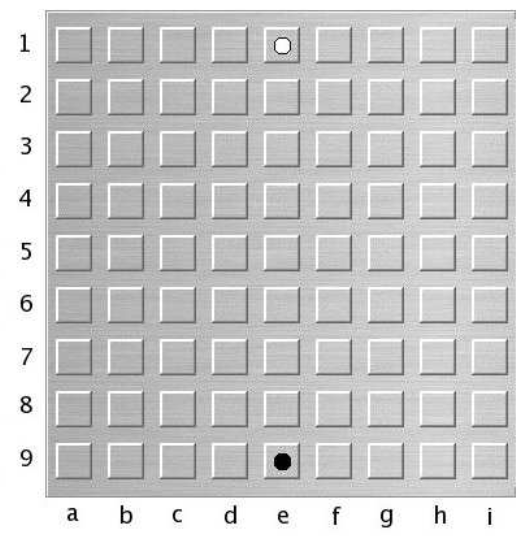
\includegraphics[scale=0.5]{blankBoard}
    \caption{Plateau de jeu }
    \label{blankBoard}
  \end{center}
\end{figure}

Le plateau de jeu ressemble  à celui de la figure~\ref{blankBoard} (extrait du 
mémoire de Glendenning, p 4). Il a une dimension de 9x9.
\\
Visuellement, les pions se placent dans les cases du plateau et les murs \og entre
deux d'entre elles \fg{} et prennent 2 places.

\subsubsection{Déroulement d'une partie}

Le Quoridor peut se jouer à 4 joueurs mais nous ne travaillerons, ici, qu'avec 2 
joueurs : un pion BLANC et un NOIR.
\\

Comme dit précédemment, les joueurs jouent chacun leur tour. Le premier à jouer est tiré 
aléatoirement. Ils ont le choix soit de se déplacer, soit de placer un mur.

\paragraph{Déplacement \\ \\}

A part quelques cas particuliers, les pions ne peuvent se déplacer que d'une case à 
la fois dans les directions cardinales (gauche, haut, droite, bas). Ils ne peuvent pas
traverser les murs.\\

Si les deux pions sont adjacents et qu'il n'y a pas de mur entre eux, le joueur dont
c'est le tour peut faire sauter son pion au dessus de son adversaire. Ce saut doit
être sur une ligne droite, à moins qu'il y ait un mur derrière l'autre pion (ou la fin du plateau), 
auquel cas le saut se fait en diagonal (voir figure~\ref{jumpMoves}).
\\

\begin{figure}[h]
  \begin{center}
    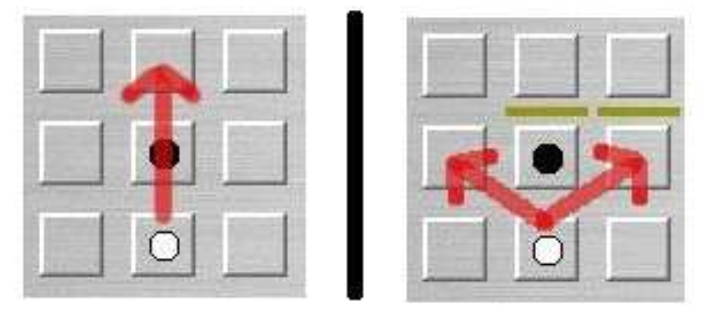
\includegraphics[scale=0.3]{jumpMoves}
    \caption{Sauts de pion autorisés}
    \label{jumpMoves}
  \end{center}
\end{figure}

\paragraph{Placement d'un mur\\ \\}

Chaque joueur possède 10 murs, il ne peut pas en placer plus. Ces murs
peuvent être placés partout sur le plateau à part quelques restrictions.
En effet, un mur ne doit pas en \og couper \fg{} un autre ni une bordure 
du plateau.
Ils se placent \og entre deux cases \fg{} du plateau soit 
verticalement, soit horizontalement.\\
Cependant, quand on place un mur, on indique uniquement une case. Si
le mur est placé en position horizontale, il sera placé en dessous de cette
case et s'il est placé en position verticale il sera à droite
(voir figure~\ref{wallplacement}).
\\

\begin{figure}[h]
  \begin{center}
    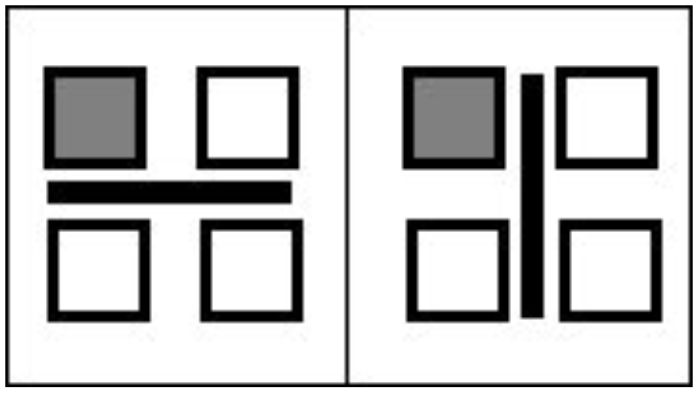
\includegraphics[scale=0.22]{wallplacement}
    \caption{Exemples de placement de murs avec la case à laquelle ils
    sont associés en gris}
    \label{wallplacement}
  \end{center}
\end{figure}

Il est interdit de bloquer complètement un pion, c'est-à-dire de placer des murs de façon à
ce qu'il ne puisse pas atteindre sa ligne d'arrivée.

\subsection{Description du serveur}

Le serveur est en quelque sorte l'\textit{arbitre} du jeu. Son r\^ole est 
d'assurer le déroulement du jeu en vérifiant que les règles sont bien 
respectées.\\

A chaque tour, le serveur \textit{donne la main} à un joueur, récupère son coup  
(déplacement ou placement d'un mur) et vérifie que ce dernier est correct. Si 
c'est cas, il passe alors la main à l'autre joueur et fait la m\^eme chose.
Et ainsi de suite jusqu'à obtenir un gagnant.\\

Un joueur gagne la partie quand il \og traverse \fg{} le plateau et arrive sur la ligne 
adverse. En revanche, si le serveur détecte une tentative de tricherie, il arr\^ete la 
partie et l'auteur de celle-ci a perdu (par exemple si un joueur tente de se déplacer 
deux fois de suite).
\\

Dans notre programme, le serveur gère également l'affichage de la partie à 
l'écran.\\

De plus, il écrit une trace de la partie dans un fichier sous le 
format décrit dans le mémoire de Glendenning (p 16). Un tel fichier ressemble
à ceci :
\begin{verbatimtab}[2]
  e8 e2
  e7 e3
  e7h e2h
\end{verbatimtab}

Dans cet exemple, le premier joueur s'est déplacé dans la case de coordonnées (E, 8)
puis son adversaire dans la case de coordonnées (E, 2).
\verb,e7h, signifie que le joueur a placé un mur horizontal en position (E, 7).

\subsection{Description des stratégies demandées}

Deux stratégies nous ont été demandées :
\begin{itemize}
\item une stratégie aléatoire
\item une stratégie \textit{MinMax}\\
\end{itemize}

Si la stratégie aléatoire ne demande pas beaucoup d'explications (à chaque tour
le joueur choisit d'effectuer un déplacement ou de placer un mur de manière aléatoire), 
le principe de la stratégie \textit{MinMax} mérite d'\^etre expliqué.
\\

Le principe régissant d'un tel algorithme est le pessimisme.
On va supposer qu'après chaque décision de notre part, notre opposant choisira 
le coup qui nous mettra dans la moins bonne position. En contrepartie, quand 
c'est à nous de jouer, on essaiera de choisir le meilleur coup pour éviter 
au maximum de se faire évincer par notre opposant.

C'est la stratégie du moins pire, qui s'avère être une bonne stratégie dans les 
jeux dit \og à sommes nulles \fg{} (les deux joueurs ne peuvent pas gagner, ou perdre
tous les 2, si l'un gagne, l'autre perd). \\

\vspace{2cm}

Ainsi, on voit bien que le jeu de \textit{Quoridor} se divise en deux grandes parties 
relativement indépendantes: 
\begin{itemize}
\item le serveur qui assure le déroulement du jeu
\item les stratégies qui jouent
\end{itemize}

\newpage

\section{Serveur}

\subsection{Structures de données}

Nous avons 3 structures différentes : 
\begin{itemize}
  \item \verb,player, : représente un joueur par ses coordonnées
  \item \verb,wall, : représente un mur par ses coordonnées et son orientation (verticale ou horizontale)
  \item \verb,board, : réprésente le plateau de jeu \\
\end{itemize}

Attardons nous un peu plus longtemps sur cette dernière structure. Elle
contient :

\begin{itemize}
  \item un tableau de deux cases de type \verb,struct player, qui représente la position des joueurs 
  \item un entier représentant le dernier joueur ayant joué
  \item un entier représentant le joueur courant (la distinction 
    étant faite avec le  dernier joueur ayant joué pour gérer le cas où un joueur 
    essaierai de jouer deux fois durant le même tour (utiliser 2 fois 
    \verb,move_pawn, successivement par exemple))
  \item les nombres de murs : nombre total (un entier) et nombre par joueurs (à l'aide d'un tableau d'entiers de taille 2)
  \item un tableau de type \verb,struct wall, contenant la position des murs \\
\end{itemize}

Cette structure est déclaré globalement, mais la portée est limitée aux fonctions 
dans le fichier d'implémentation du serveur (\verb,interface.c,), pour que les 
stratégies n'y ait pas accès facilement. Le mot clé \verb,static, est ici utilisé pour
le garantir.

\subsection{Un choix de représentation optimal ?}

Le choix de stocker la position des murs est trés discutable pour 
l'implémentation algorithmique. En effet, à chaque fois qu'on veut tester s'il y 
a un mur adjacent à une case du plateau donnée, il faudra parcourir le 
tableau de murs.

Il faudrait donc a priori plus de temps pour le faire que si on avait stocké dans une 
matrice, la présence ou non d'un mur pour chaque case du plateau. Cependant, nous 
n'avons pas mesurer les temps moyens d'éxecution de ces deux configurations pour pouvoir 
réellement confirmer l'éventuel problème.\\

A noter que cette dernière solution a été choisie dans la stratégie \textit{MinMax}.
En effet, elle nécessite un plateau propre à elle pour pouvoir simuler des coups à 
l'avance.

\subsection{Interface}

\subsubsection{A quoi sert l'interface ?}

Comme son nom l'indique, l'interface fait le lien entre le serveur et les stratégies 
des joueurs. En effet, les fonctions fournies par l'interface sont le seul moyen pour
les stratégies de \og communiquer \fg{} avec le serveur (demander l'état du plateau 
et lui envoyer ses coups).

\subsubsection{Présentation des fonctions disponibles}

Les prototypes des fonctions de l'interface nous ont été imposés pour assurer une 
compatibilité avec les stratégies. Nous les avons donc conserver. Cependant, nous 
avons fait le choix de ne pas utiliser le pointeur passé en paramètre dans 
les fonctions de l'interface (puisque que nous avons une structure globale, les 
fonctions implémentant notre serveur peuvent opérer directement dessus.)\\

Toutefois, les éventuelles stratégies concurrentes ne devront  pas s'étonner de 
se voir passer pour paramètre \verb:struct board *b: un pointeur  arbitrairement 
fixé à la valeur \verb,NULL,. Celle ci peuvent même s'amuser à changer complètement la 
valeur envoyée au serveur via l'interface car cette valeur sera totalement 
ignorée.\\

Cette interface propose :
\begin{itemize}
\item \verb,get_current_player, : une fonction permettant de récupérer l'identifiant du joueur courant
\item \verb,get_position, :  une fonction permettant de conna\^itre le contenu d'une case : contient le
  pion BLANC, le pion NOIR ou rien
\item \verb,is_passable, : une fonction permettant de savoir si un déplacement à partir d'une case donnée vers 
  une direction donnée est possible
\item \verb,move_pawn, : une fonction permettant de déplacer un pion en donnant les coordonnées de sa destination
\item \verb,remaining_bridges, : une fonction permettant de conna\^tre le nombre de murs qu'il nous reste (attention, le nom de cette fonction est assez trompeur : \verb,remaining_bridges, alors qu'on parle de murs)
\item \verb,is_blockable, : une fonction permettant de savoir s'il est possible de placer un mur à une case et une orientation données
\item \verb,place_wall, : une fonction permettant de placer un mur en donnant ses coordonnées et son orientation
\end{itemize}

\subsubsection{Vérification de la validité des coups}

Nous rappelons que le serveur doit vérifier que les coups effectués par les stratégies 
sont corrects. Nous remarquons que seules les fonctions \verb,move_pawn, et 
\verb,place_wall, \og modifient \fg{} le plateau de jeu. En réalité, celui-ci est modifié 
seulement si le coup est valide.
\\

En effet, nous ne nous contentons pas mettre le plateau à jour sans regarder ce que les 
stratégies nous envoient, mais nous vérifions que ce coup est bien valide.

\subsection{Mise en \oe uvre}

Ainsi, nous venons de voir que les deux fonctions principales du serveur de jeu sont les 
suivantes:
\begin{itemize}
  \item le calcul de la validité d'un coup : \og placement d'un mur \fg{}
  \item le calcul de la validité d'un coup : \og déplacement du pion \fg{}
\end{itemize}

\subsubsection{Calcul de la validité du placement d'un mur}

Ces problèmes se découpent en sous-problèmes. Par exemple, le premier 
peut se découper comme suit:
\begin{itemize}
  \item calculer si un mur n'est pas déja posé dans la position donnée
  \item calculer si le mur à poser ne rencontre pas et/ou ne se superpose pas 
partiellement à un mur déja posé
  \item calculer si le mur n'emp\^eche pas définitivement au moins l'un des deux 
joueurs d'atteindre sa ligne d'arrivée \\
\end{itemize}

C'est le dernier point qui requiert le plus de calcul. On en vient à bout, en 
considérant le plateau comme un graphe (voir A Quoridor Playing Agent, Mertens 
figure 9 p.4) et en effectuant un parcours en profondeur :
depuis une case, on visite toutes les cases voisines, et on ne repasse jamais par une 
case déja visitée.\\

Cet algorithme est terminé dès qu'il rencontre une case appartenant à la ligne 
d'arrivée du joueur, auquel cas on peut poser le mur. Cepedant, lorsque qu'il a 
parcouru tout le graphe accessible sans réussir à atteindre cette ligne 
d'arrivée, poser un mur est interdit.\\

La complexité de cette algorithme est en $\mathcal{O}($ \text taille plateau 
$)$.

\subsubsection{Calcul de la validité du déplacement d'un pion}

Le deuxième problème se découpe comme suit:
\begin{itemize}
  \item le joueur décide de se déplacer en diagonale
  \item le joueur décide de se déplacer de deux cases en ligne droite
  \item le joueur décide de se déplacer de manière classique. \\
\end{itemize}

La difficulté ici est de trouver quel sera le meilleur découpage possible pour 
réussir à écrire des algorithmes simples venant à bouts des problèmes. Le choix 
de la structure de données peut aussi être déterminante dans ces choix.

\subsection{Affichage de la partie}

Comme nous l'avons dit précédemment, notre serveur s'occupe également d'afficher 
le déroulement de la partie à l'écran. Cet affichage est réalisé dans le terminal 
grâce à la librairie \texttt{ncurses}. \\

Nous avons choisi de garder un affichage très simple pour avoir plsu de temps à
consacrer à la réalisation des stratégies.\\

Un aperçu du rendu du plateau est présenté en figure~\ref{fig:plateau_ncurses}. \\
\begin{figure}[h!]
  \begin{center}
    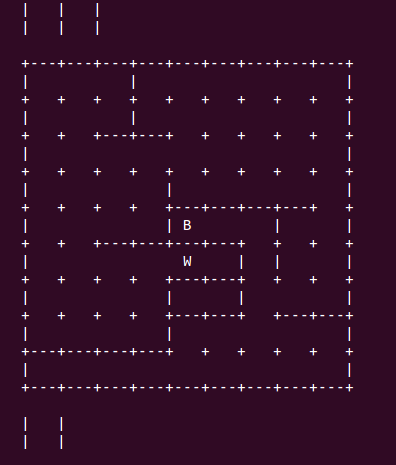
\includegraphics[scale=0.45]{plateau}
	\caption{Plateau de jeu}
	\label{fig:plateau_ncurses}
  \end{center}
\end{figure}

\newpage
Les différentes fonctions réalisant l'affichage de notre plateau sont 
implémentés dans le fichier \verb,display.c,.

\section{Stratégies}

\subsection{Aléatoire}
\subsubsection{Description}
La stratégie aléatoire est très simple : elle tire un coup un hasard et demande 
au serveur si le coup est valide ou si le coup ne convient pas, via l'interface  
(\verb,is_passable,,
 \verb,get_position, et \verb,is_blockable,).
Tant que le coup ne convient pas, elle recommence et tire à nouveau un coup au 
hasard.

\subsubsection{Problèmes}

La réalisation cette première stratégie aléatoire est basique, peut-etre même 
un peu trop.\\

Le choix du mouvement du joueur se fait en choissisant une des quatres 
directions cardinales au hasard, en regardant s'il n'y a pas de murs dans cette 
direction puis si la case n'est pas occupée (elle ne gère pas les sauts par 
dessus l'ennemi).\\

Que se passe-t-il lorsque le joueur se retrouve dans un cul  de sac, que le 
joueur  ennemi lui fait face, et que c'est à son  tour de jouer? La partie se 
bloque (voir \verb,./tst/test_random_strategy,).\\

\subsection{\textit{MinMax}}

\subsubsection{Principe et condition nécessaire à son fonctionnement}

La réalisation de la stratégie \textit{MinMax} a été plus délicate.
Pour mener à bien la prise d'une décision par un algorithme \textit{MinMax}, il faut à 
priori calculer dans un premier temps l'ensemble des coups possibles pour un 
joueur à partir d'un état du plateau donné.\\

La stratégie minimax est récursive et s'applique jusqu'à une certaine 
profondeur de récursion sur tous les états possibles du jeux à partir d'un état 
initial.\\

\noindent Ainsi, dans un premier temps, les étapes de l'algorithme sont :
\begin{enumerate}
  \item calcul de tous les coups possibles
  \item stockage de chaque coup dans une structure \verb,Move,
  \item ajout de chacun des coups possibles dans une liste chainée (dynamique car on ne 
    sait pas, selon l'état du jeu, le nombre de coups possibles, ce dernier dépend 
    aussi du nombre de murs que l'on peut placer)
  \item parcourt de cette liste pour appeler la stratégie \textit{MinMax} sur chacun d'eux.\\
\end{enumerate}

La figure~\ref{algo} décrit en pseudo-code cet algorithme.

\begin{figure}[h]
\begin{verbatimtab}[2]
fonction minimax(noeud N = coup, entier profondeur, booleen JoueurEnnemi): 
valeur
debut
	si profondeur = 0
		retourner evaluation(N);

	tant que il existe un coup possible
		ajouterElement(ListeCoup, prochainCoupPossible)
	fin de tant que
	
	si JoueurEnnemi
		a <- +infini
		pour chaque element de la liste
			a <- min(a, minimax(element, profondeur-1, non(JoueurEnnemi))
		fin pour
		retourner a
	sinon
		a <- -infini
		pour chaque element de la liste
			a <- max(a, minimax(element, profondeur-1, non(JoueurEnnemi))
		fin pour
		retourner a
	fin si
fin
  \end{verbatimtab}
  \caption{Première version algorithme MinMax}
  \label{algo}
\end{figure}

\subsubsection{Problème de complexité}

La complexité du \textit{MinMax} est exponentielle, la base de l'exponentielle étant le 
nombre de coups possibles à partir d'un coup donné. On appelle aussi ce nombre 
\og \textit{branching factor} \fg{}, à savoir le nombre de fils pour chaque noeud de l'arbre des
possibilités du jeu\footnote{Glendenning thesis p.70} (cette quantité étant variable entre 133 et 1 une mesure pertinente de 
celle-ci est sa moyenne, évaluée à environ 60).\\

Sur un ordinateur lent, cette complexité se fait 
extr\^emement ressentir lorsque que l'on passe de la profondeur 2 à la profondeur 
3 pour \textit{MinMax}. La durée du calcul passe de 1-2 seconde(s), à une 
durée comprise entre 1 et 2 minutes.\\

La profondeur de 3 a toutefois été retenue car le calcul se fait en un temps tout 
à fait respectable sur des machines du calibre de celles de l'Enseirb.\\

Calculer si un coup est autorisé prend du temps (en particulier calculer si l'on 
est autorisé à placer un mur, puisque qu'il faut verifier si l'on ne bloque pas 
definitivement l'un des  joueurs, et donc parcourir le plateau quasiment en 
entier).\\

Calculer la valeur d'un coup prend également du temps: lorsque que l'on arrive à 
la profondeur maximale, on arrête les  appels récursifs et on évalue la 
situation gr\^ace à la fonction d'évaluation. Celle-ci est appelée sur chacune des 
feuilles ($60^n$ fois pour une profondeur $n$), sa complexité est donc critique 
pour la complexité globale de \textit{MinMax}.\\

\subsubsection{Alpha Beta}

Il existe une amélioration de l'algorithme \textit{MinMax} appelé \og élagage 
alpha-beta \fg{} qui 
permet, comme son nom l'indique, d'élaguer l'arbre des possibilités en 
remarquant que le parcours de certaines  branches de l'arbre est inutile dans le 
calcul de \textit{MinMax}. 
\\

Nous nous sommes rendu compte qu'en fait, avant de commencer le premier appel récursif de 
\textit{MinMax}, au lieu de calculer si différents 
coups possibles étaient valides, on pouvait les calculer au fur et à mesure. Nous
profiterions ainsi au maximum du  
gain de temps apporté par l'amélioration alpha-beta. \\

Nous avons donc choisi, dans un second temps, de caculer si un coup est possible puis de directement appeler le 
\textit{MinMax} sur ce \og fils \fg{} (le coup) pour obtenir sa valeur (le \textit{MinMax} associe une 
valeur à chaque noeud). On peut ainsi tout de suite voir si une coupure (un élagage) 
est possible, et ce avant même de conna\^itre tous les coups autorisés pour l'état 
actuel du jeu. 
\\

Ce nouvel algorithme est donné en figure~\ref{algo2}.

\newpage
\begin{figure}[h]
\begin{verbatimtab}[2]
Fonction minimax(noeud N = coup, entier profondeur, booleen JoueurEnnemi
valeur alpha, valeur beta): valeur
debut
	si profondeur = 0
		retourner evaluation(N);

	si JoueurEnnemi
		tant que des coups sont possibles
			coup <- prochainCoupPossible();
			alpha <- min(alpha, minimax(coup, profondeur-1, non(JoueurEnnemi),
						alpha, beta);
			si coupePossible(alpha, beta)
				retourner alpha;
		fin tant que
		retourner alpha;
	sinon
		a <- -infini;
		idem avec max et alpha<->beta ....
		retourner beta
	fin si
fin
  \end{verbatimtab}
  \caption{Deuxième version algorithme MinMax}
  \label{algo2}
\end{figure}

\subsubsection{Fonction d'évalutation}

Nous avons pris du temps pour lire les documents de Mertens et de Glendening, et nous
nous sommes beaucoup inspiré de leur travail pour choisir notre fonction d'évaluation. 
\\
 
Les différents paramètres que nous avons retenus sont:
\begin{itemize}
  \item plus courte distance (en nombre de déplacements) pour que le joueur 
    appelant la stratégie atteignent sa ligne d'arrivée
  \item différence entre le nombre de coups pour gagner pour les deux joueurs
  \item un peu d'aléatoire.
\end{itemize}

\newpage 

\section{Résultats obtenus}

\subsection{Compiler et exécuter notre programme}

Nous allons tout d'abord vous donner la marche suivre pour pouvoir compiler
et exécuter notre programme. Nous supposons que la machine sur laquelle sera
compilé notre programme tourne sous un système \texttt{UNIX} et possède toutes 
les bibliothèques nécessaires.
\\

Voici les étapes à suivre :
\begin{enumerate}
  \item se placer dans le dossier \texttt{s5-quor-1021/} (\verb,cd s5-quor-1021,)
  \item lancer le \texttt{Makefile} (commande \texttt{make}) 
  \item lancer le programme avec la commande \texttt{./bin/quoridor} \\
\end{enumerate}

\subsection{Batterie de tests}

Nous fournissons également une batterie de tests unitaires dont les sources sont
 disponibles dans le dossier \verb,tst/,.\\

Si vous avez suivi la démarche de la sous-section précédente, les tests sont déjà compilés
(vous pouvez néanmoins les recompiler en faisant un \verb,make, depuis le dossier 
\texttt{s5-quor-1021/}). \\

Il suffit alors de lancer la commande suivante depuis le dossier 
\texttt{s5-quor-1021/} : \\
\verb,./bin/test_quoridor,\\

Le dossier \verb,tst/, contient également la mise en évidence d'un problème de la stratégie 
aléatoire. Pour le lancer :\\
\verb,./tst/test_random_strategy,\\

\subsection{Jeu d'essai}

Au lancement du programme (\verb,./bin/quoridor,), vous devriez avoir un écran qui ressemble à cela (figure~\ref{acc}) :

\begin{figure}[h]
  \begin{center}
    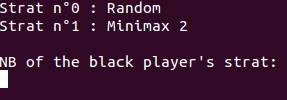
\includegraphics[scale=0.7]{acc}
    \caption{Ecran d'accueil}
    \label{acc}
  \end{center}
\end{figure}

Vous pouvez alors choisir parmi nos deux stratégies en tapant soit $0$ (pour la stratégie aléatoire) soit $1$ (pour \textit{MinMax}). Une fois que vous avez choisi vos deux stratégies, le jeu se lance. Nous vous conseillons d'agrandir un peu votre terminal pour avoir un affichage optimal. \\

La figure~\ref{jeu} montre le déroulement d'une partie à un instant donné.\\

\begin{figure}[h]
  \begin{center}
    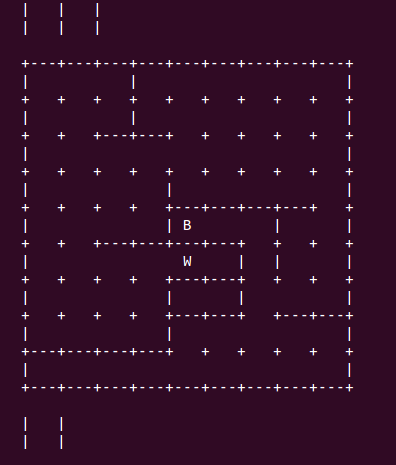
\includegraphics[scale=0.7]{plateau}
    \caption{Déroulement d'une partie à un instant donné}
    \label{jeu}
  \end{center}
\end{figure}

Le \verb,B, représente le pion NOIR (\og BLACK \fg{}) et le \verb,W, le pion BLANC (\og WHITE \fg{}). On voit qu'il reste encore 2 murs au joueur NOIR et 3 au joueur BLANC.

\newpage
\section*{Conclusion}

A la fin de ces 7 semaines de projet, nous sommes contents des résultats que nous avons 
obtenus. Le cahier des charges est rempli puisque nous avons :
\begin{itemize}
  \item un serveur qui fonctionne bien, à savoir :
    \begin{itemize}
      \item[.] qui fait jouer deux stratégies
      \item[.] qui vérifie la validité des coups
      \item[.] qui affichage le déroulement de la partie à l'écran
    \end{itemize}
  \item deux stratégies :
    \begin{itemize}
      \item[.] aléatoire
      \item[.] \textit{MinMax} \\
    \end{itemize}
\end{itemize}

De plus, ce premier projet nous a permis d'appliquer de manière concrète les notions d'algorithme et de programmation impérative que nous avons vu en cours. Il était également très intéressant de travailler par groupe de 3, ce qui a renforcé notre esprit d'équipe.

\end{document}
